\subsection{Конкретный синтаксис}
Для задания конкретного синтаксиса в среде \MPS{} предусмотрен проблемно"=ориентированный язык \term{jet\-bra\-ins.mps.lang.ed\-it\-or}. Он позволяет для каждого концепта определить редактор, описывающий представление узлов этого концепта в виде набора ячеек. Каждая ячейка редактора соответствует ключевому слову, свойству, вложенному узлу, ссылке или другому члену концепта. Например, для концепта \term{StateMachine} определение редактора приведено на рисунке \ref{fig:StateMachineEditor}.

\begin{figure}
 \centering
 \fbox{
  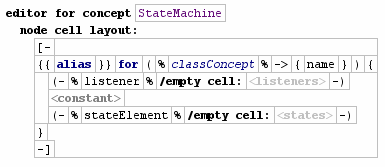
\includegraphics[width=0.9\textwidth]{StateMachineEditor.png}
 }
 \caption{Редактор для концепта \term{StateMachine}}
 \label{fig:StateMachineEditor}
\end{figure}

\begin{enumerate}
\item Конструкция "<[- ... -]"> --- составная ячейка. Она используется для того, чтобы задать конкретное представление узла концепта \term{StateMachine} в виде набора ячеек. В этом представлении никакой текст для нее выводиться не будет.
\item Ячейка "<\{\{alias\}\}"> соответствует мета"=свойству \term{alias} концепта \term{StateMachine}. Значением этого мета"=свойства, как было указано ранее, является строка "<state machine">. Таким образом, конкретное представление узлов концепта \term{StateMachine} начинается с ключевого слова "<state machine">. Для каждой ячейки 
\MPS{}"=редактора можно задать стиль. В частности, для первой ячейки задан стиль ключевого слова из языка \term{baseLanguage}.
\item В ячейке "<for"> указан текст, который будет безусловно выводиться на второй позиции.
\item Ячейка "<(\%classConcept\% -> \{name\})"> описывает представление ссылки с ролью \term{classConcept}. Вложенная ячейка "<\{name\}"> определяет то, что в качестве представления ссылки будет использовано значение свойства \term{name} того узла, на который указывает ссылка.
\item Ячейка "<\{"> соответствует открывающейся фигурной скобке.
\item Ячейка "<(-\%listener\% /empty cell: <listeners>-)"> соответствует вложенным узлам с ролью \term{listener}. На место этой ячейки будут вставлены конкретные представления вложенных узлов. Причем для каждого вложенного узла будет использован соответствующий его концепту редактор. Если у некоторого данного узла \term{StateMachine} нет вложенных узлов с ролью \term{listener}, то будет выведен текст "<<listeners>">.
\item Ячейка "<<constant>"> --- пустая ячейка без текста, в данном случае она соответствует пустой строке.
\item Ячейка "<(-\%stateElement\% /empty cell: <states>-)"> аналогично соответствует вложенным узлам с ролью 
\term{stateElement}.
\item Ячейка "<\}"> --- закрывающаяся фигурная скобка.
\end{enumerate}

На рисунке \ref{fig:EmptyStateMachine} приведен пример конкретного представления узла концепта \term{stateMachine} с двумя состояниями. Данный узел описывает автоматное поведение класса \term{SomeStatefulClass}. Узлы, соответствующие его состояниям, имеют роль \term{stateElement}.

\begin{figure}
 \centering
 \fbox{
  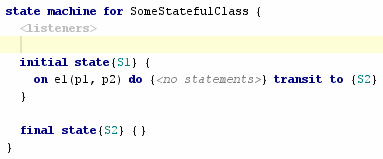
\includegraphics[width=0.9\textwidth]{EmptyStateMachine.png}
 }
 \caption{Представление узла концепта \term{stateMachine} с двумя состояниями}
 \label{fig:EmptyStateMachine}
\end{figure}
